\documentclass{beamer}

\usepackage[english]{babel}
\usepackage[utf8x]{inputenc}
\usepackage[T1]{fontenc}
\usepackage{graphicx}
\usepackage[colorinlistoftodos]{todonotes}
\usepackage{enumerate}
\usepackage{subfig}
\usepackage{ctex}
\usepackage{listings}
\usepackage{xcolor}

\title{Introduction to elgooG Search Engine}
\author{Zhipeng Chen}
\date{July 20, 2020}

\begin{document}

\maketitle

\begin{frame}
	\frametitle{Initial interface}
	\begin{center}
		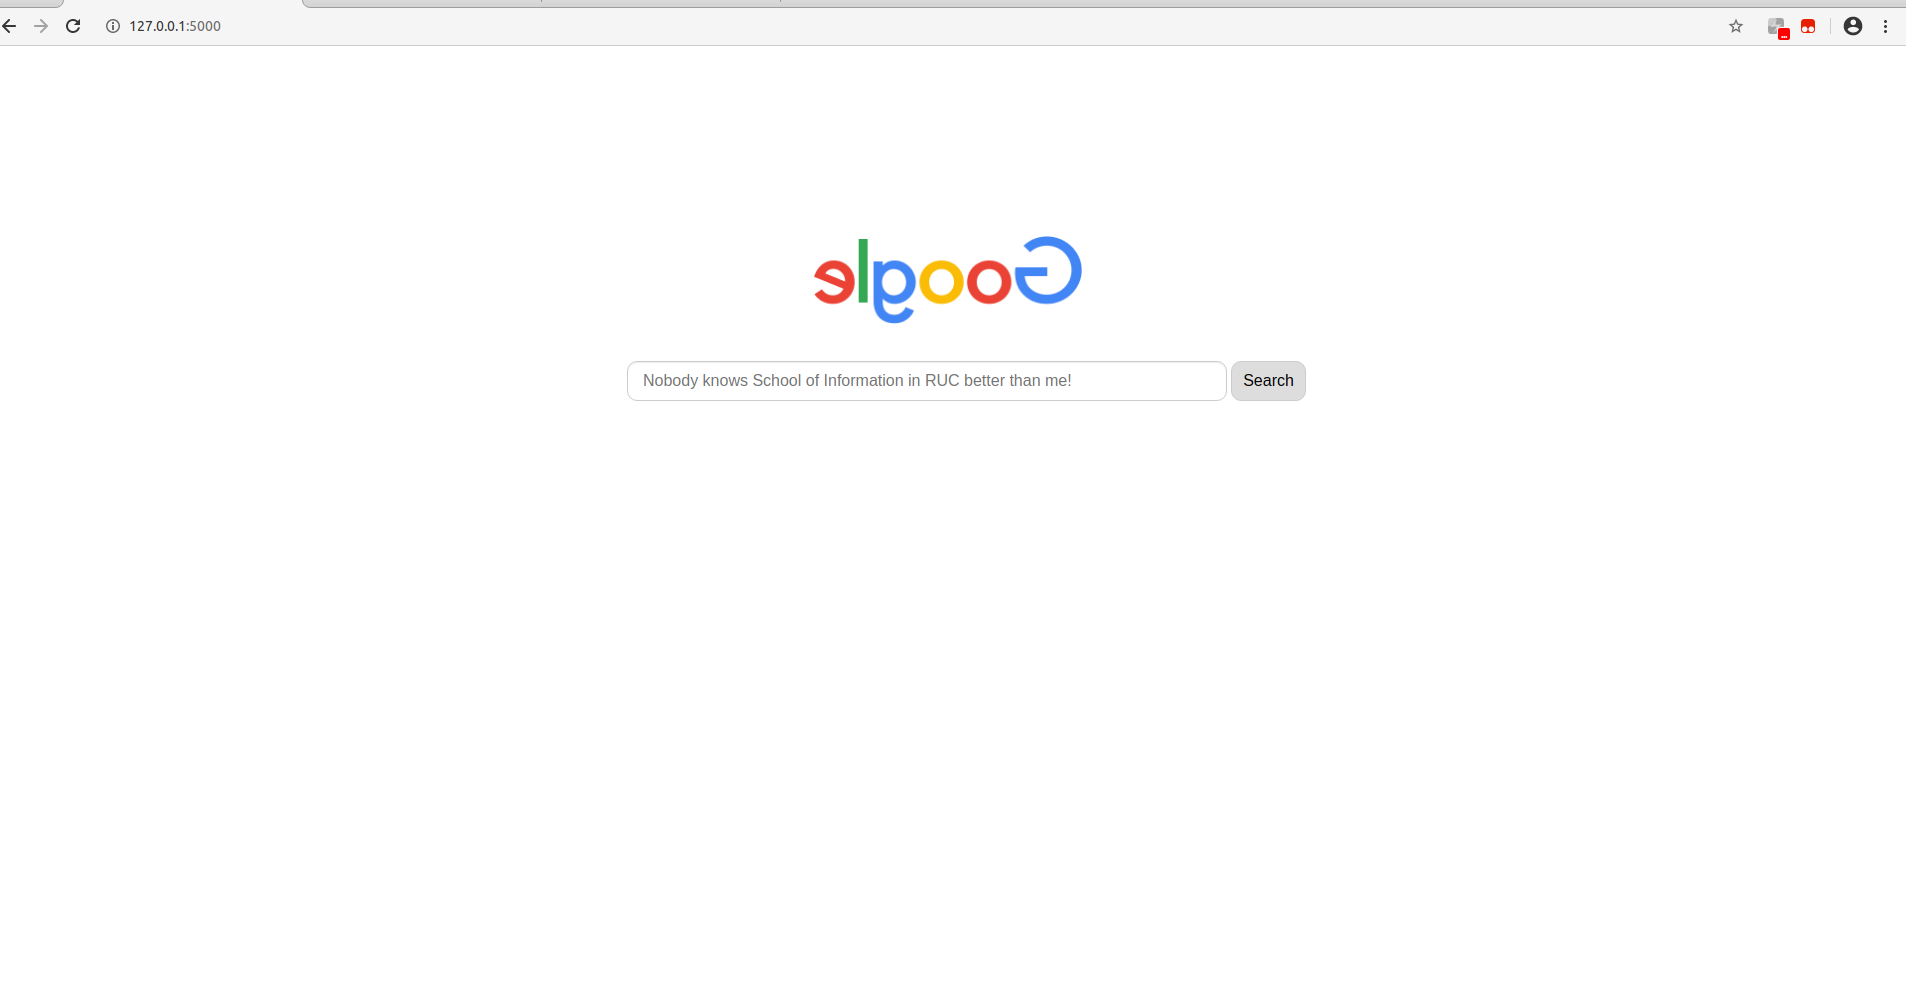
\includegraphics[width=1\textwidth, height=0.6\textheight]{UI-1.png}
	\end{center}
	
\end{frame}

\begin{frame}
	\frametitle{Result interface}
	\begin{center}
		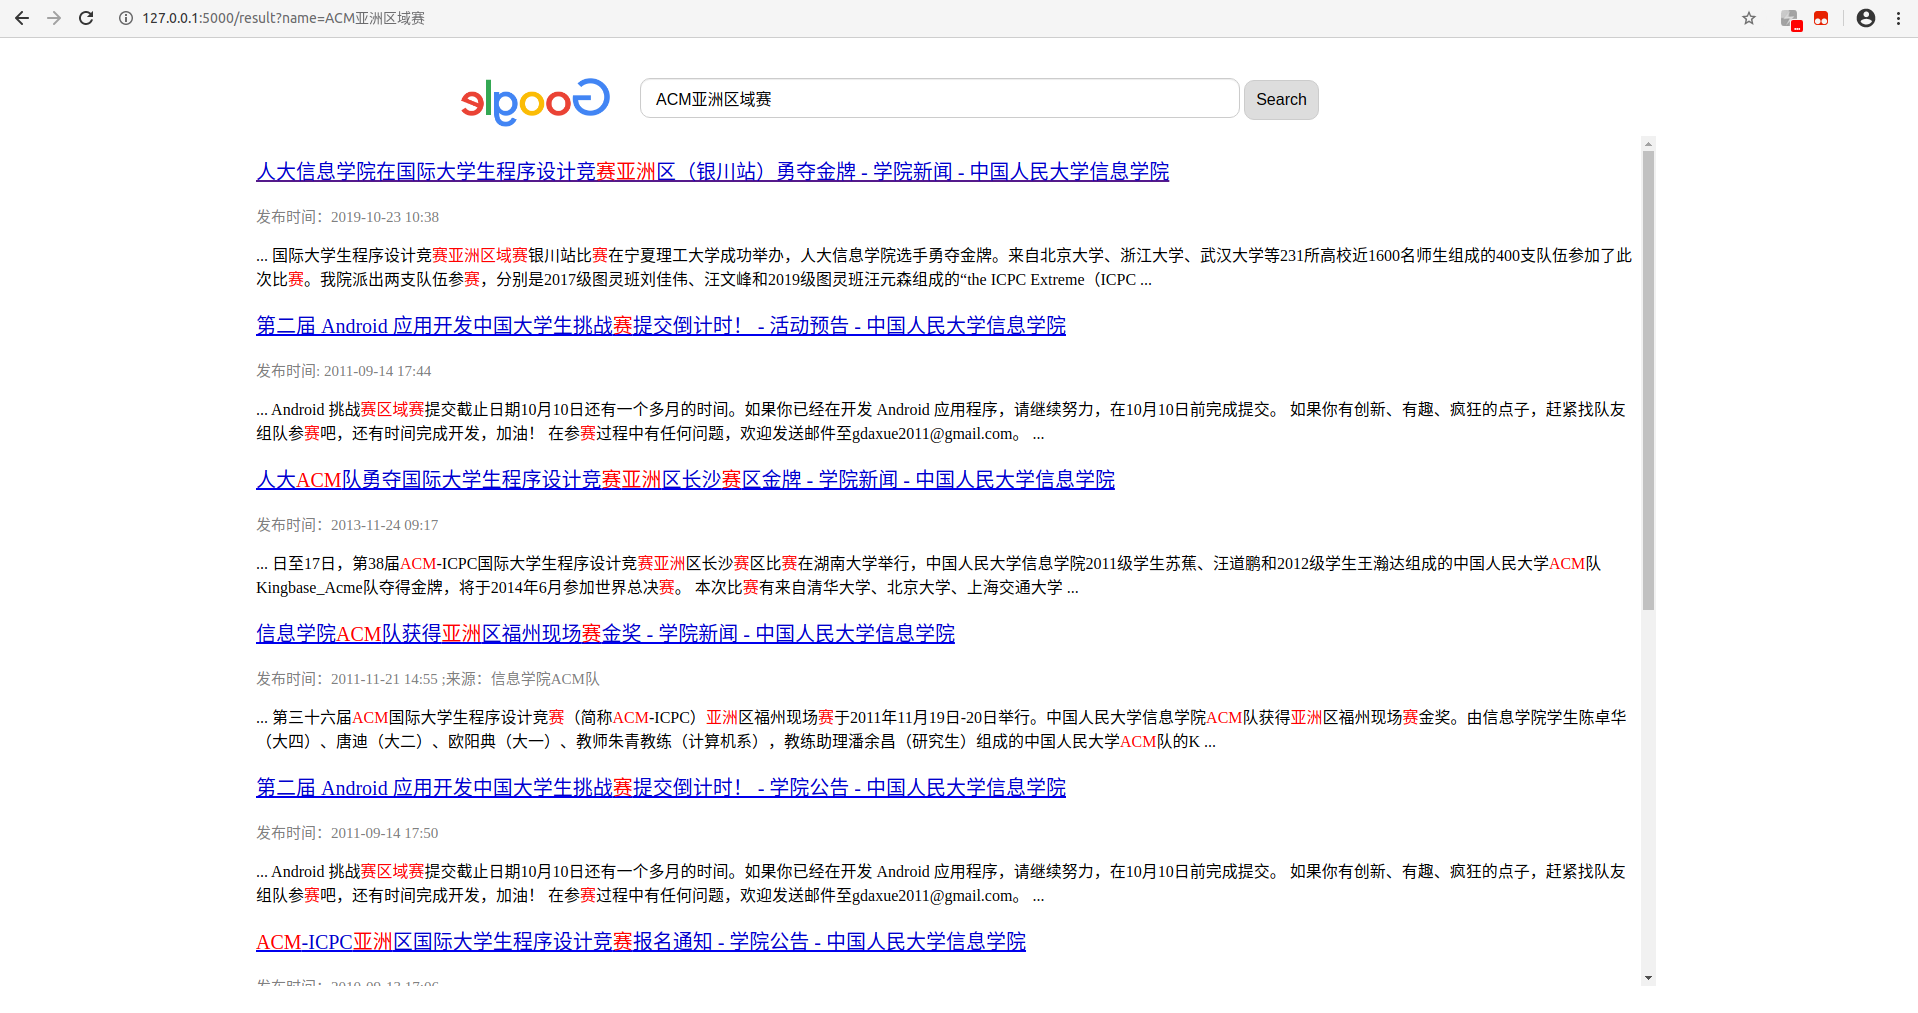
\includegraphics[width=1\textwidth, height=0.6\textheight]{UI-2.png}
	\end{center}
\end{frame}

\begin{frame}
	\frametitle{How to make it}
	(1) Crawler
	\\ \hspace*{\fill} \\
	(2) Normalized and divided
	\\ \hspace*{\fill} \\
	(3) Build the inverted index
	\\ \hspace*{\fill} \\
	(4) Solve queries

\end{frame}

\begin{frame}
	\frametitle{Optimization}
	(1) The value of word is related to the times that the word appears in website, and it also related to the lenght of the word.
	\\ \hspace*{\fill} \\
	$Value_{i,id} = (1 + \lg(t_{i,id})) * (\lg(\frac{N}{n_{id}}))^{1.75} * (\lg(len_{id}+1))$
	\\ \hspace*{\fill} \\
	(2) The value of word is related to whether it is a number.
	\\ \hspace*{\fill} \\
	$Value_{i,id} = (Value_{i,id})^{'} * (\lg(len_{id} + 1) + 1.6)$
\end{frame}

\begin{frame}
	\frametitle{Optimization}
	(3) The sorce of website is related to the lenght.
	\\ \hspace*{\fill} \\
	\begin{center}
		$Lenght_i = \sqrt{\sum{({\lg{t_{i,id}}})^2}}$
		\\ \hspace*{\fill} \\
		$Sorce_i = {Sorce_i}^{'} / {lenght_i}^{0.495}$
	\end{center}
		
\end{frame}

\begin{frame}
	\frametitle{Optimization}
	(4) Different websites have different weight.
	\\ \hspace*{\fill} \\
	If the page is about prefessor: 
	
	\begin{center}
		$Sorce_i = {Sorce_i}^{'} * 1.6 $
	\end{center}
	
	If the page is about laboratory or the overview of School of Information: 
	
	\begin{center}
		$Sorce_i = {Sorce_i}^{'} * 1.2 $
	\end{center}
	
	If the page is about news or notice: 
	
	\begin{center}
		$Sorce_i = {Sorce_i}^{'} / 1.2 $
	\end{center}

\end{frame}

\begin{frame}
	\frametitle{Example-1}
	\begin{center}
		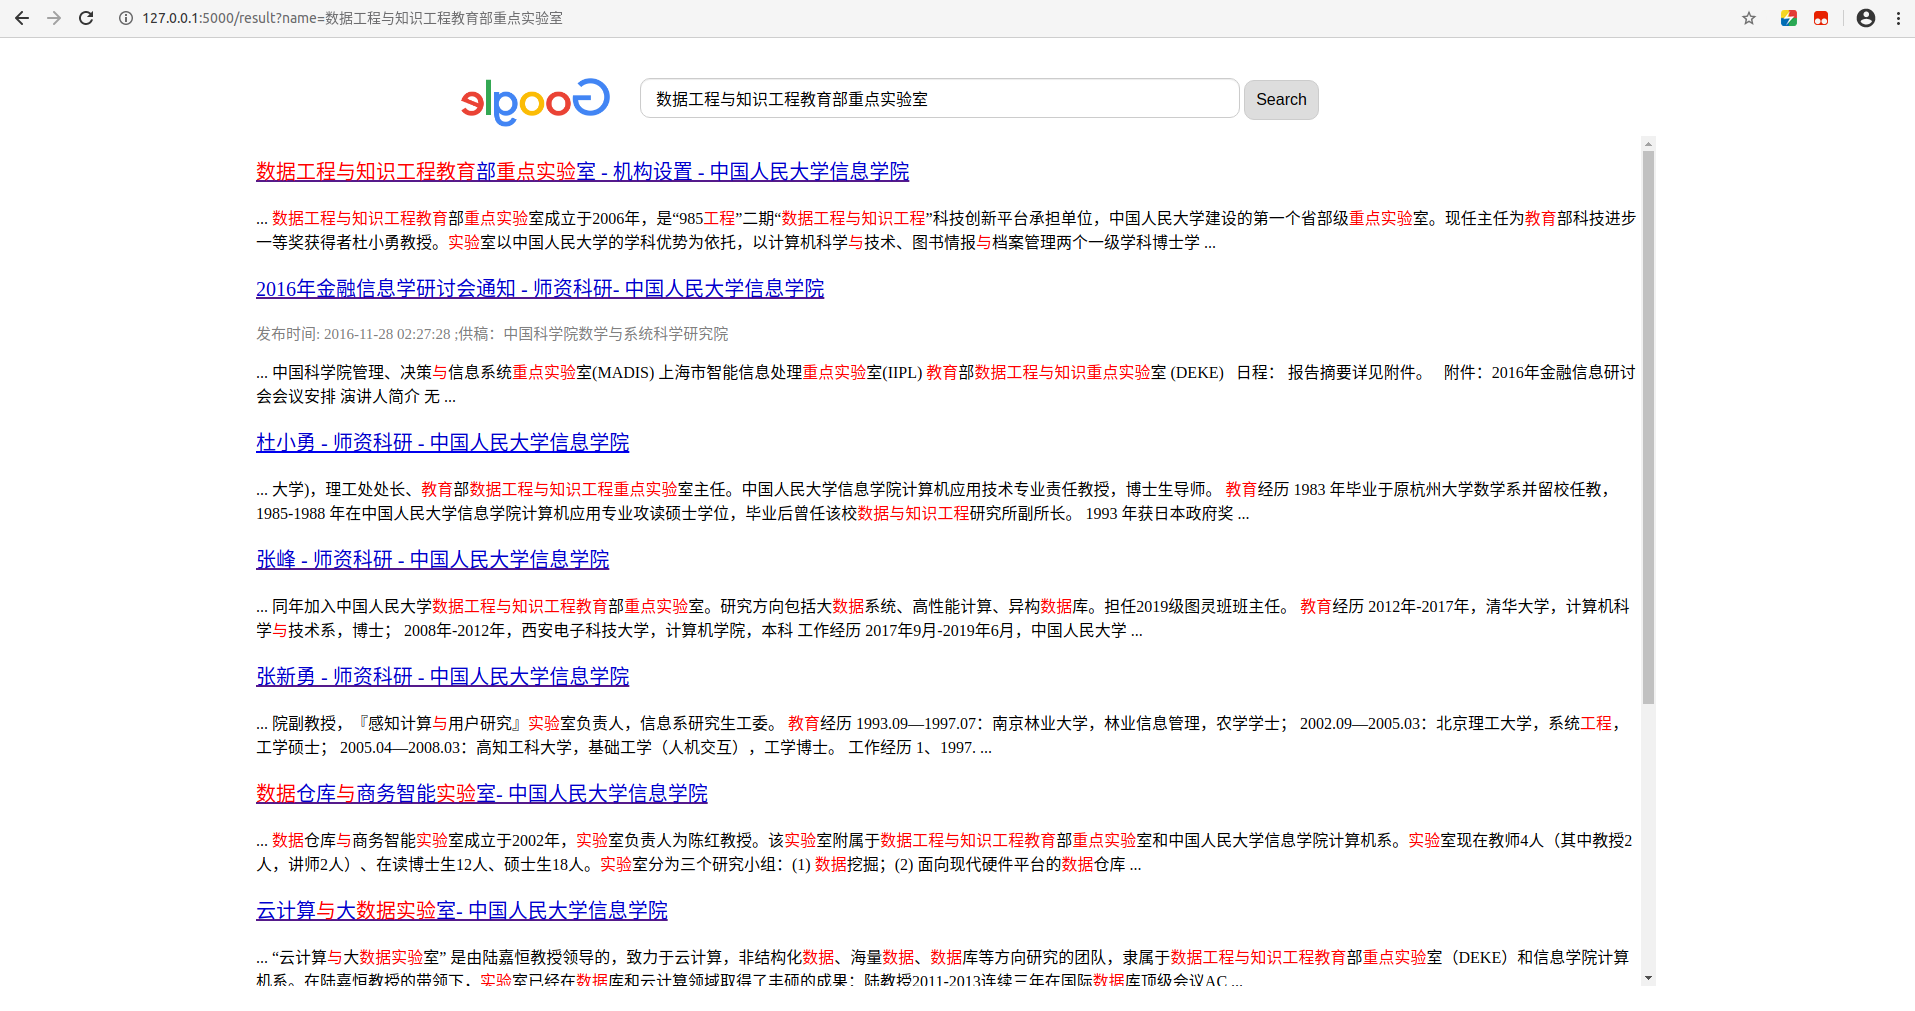
\includegraphics[width=1\textwidth, height=0.6\textheight]{example4.png}
	\end{center}
\end{frame}

\begin{frame}
	\frametitle{Example-2}
	\begin{center}
		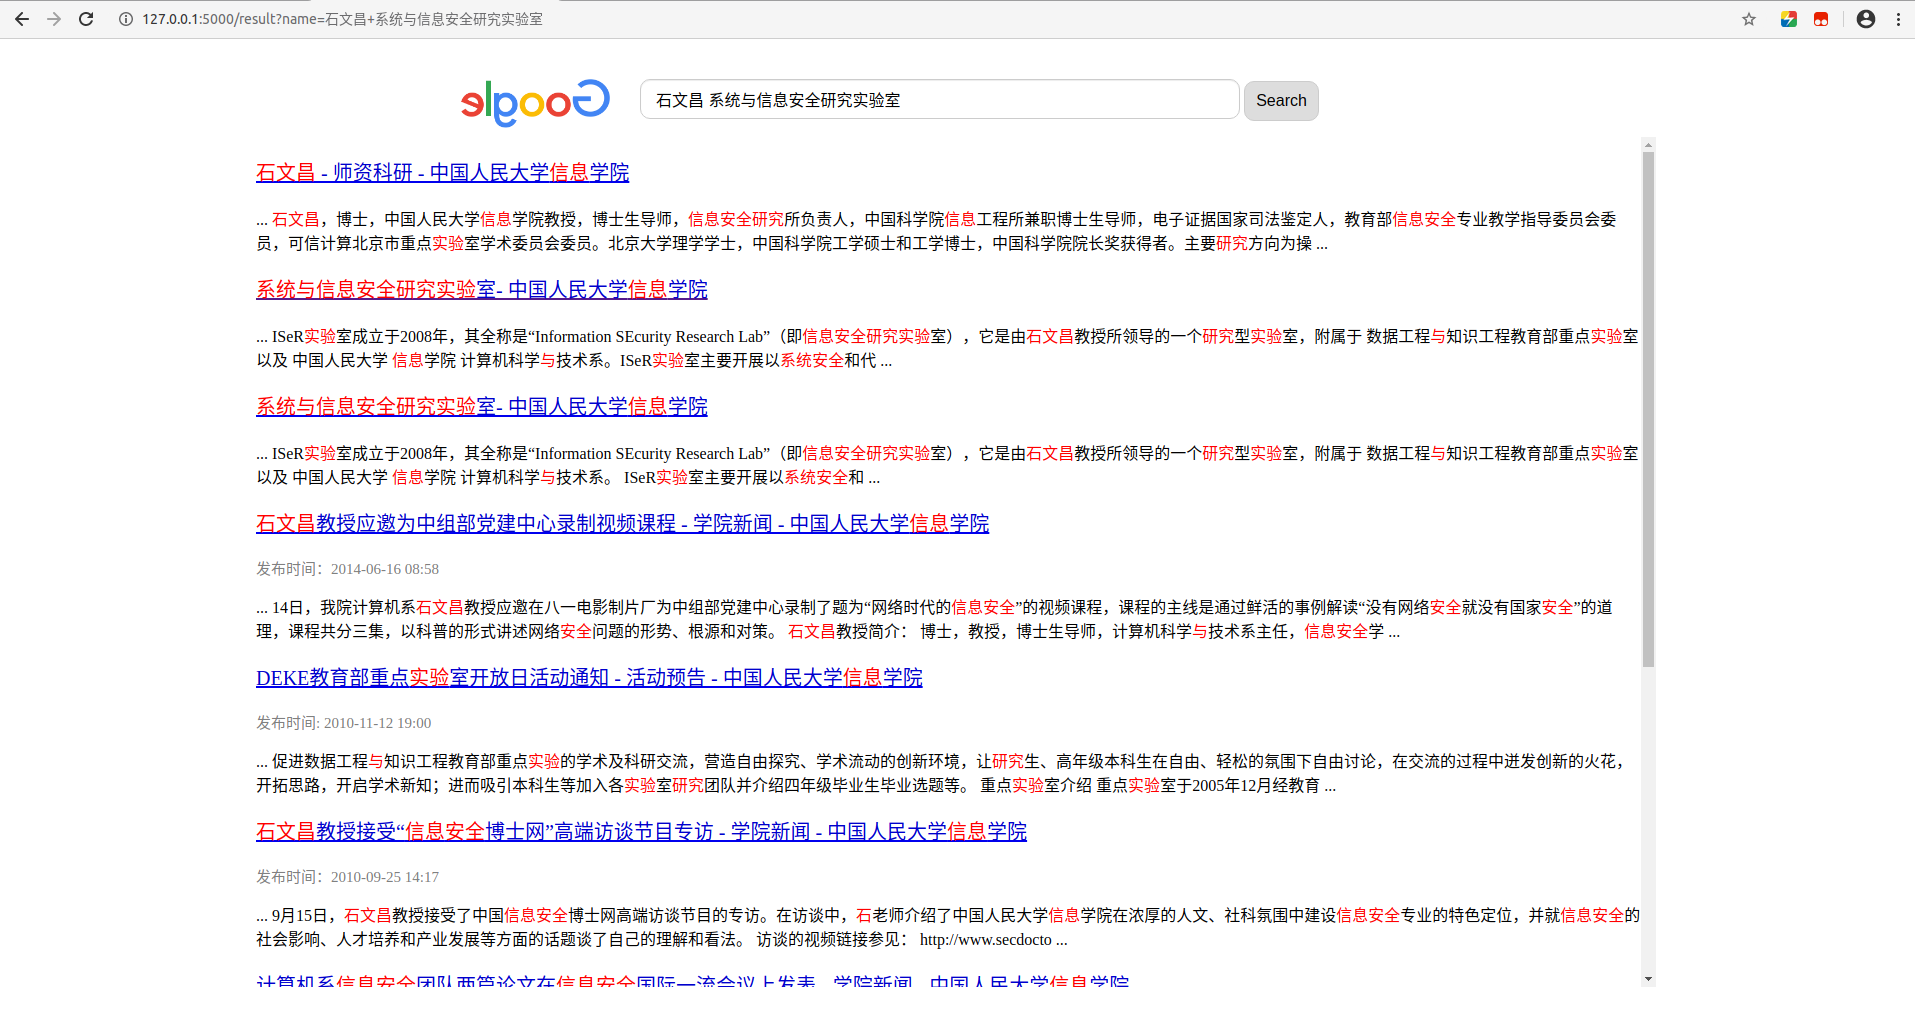
\includegraphics[width=1\textwidth, height=0.6\textheight]{example1.png}
	\end{center}
\end{frame}

\begin{frame}
	\frametitle{Example-3}
	\begin{center}
		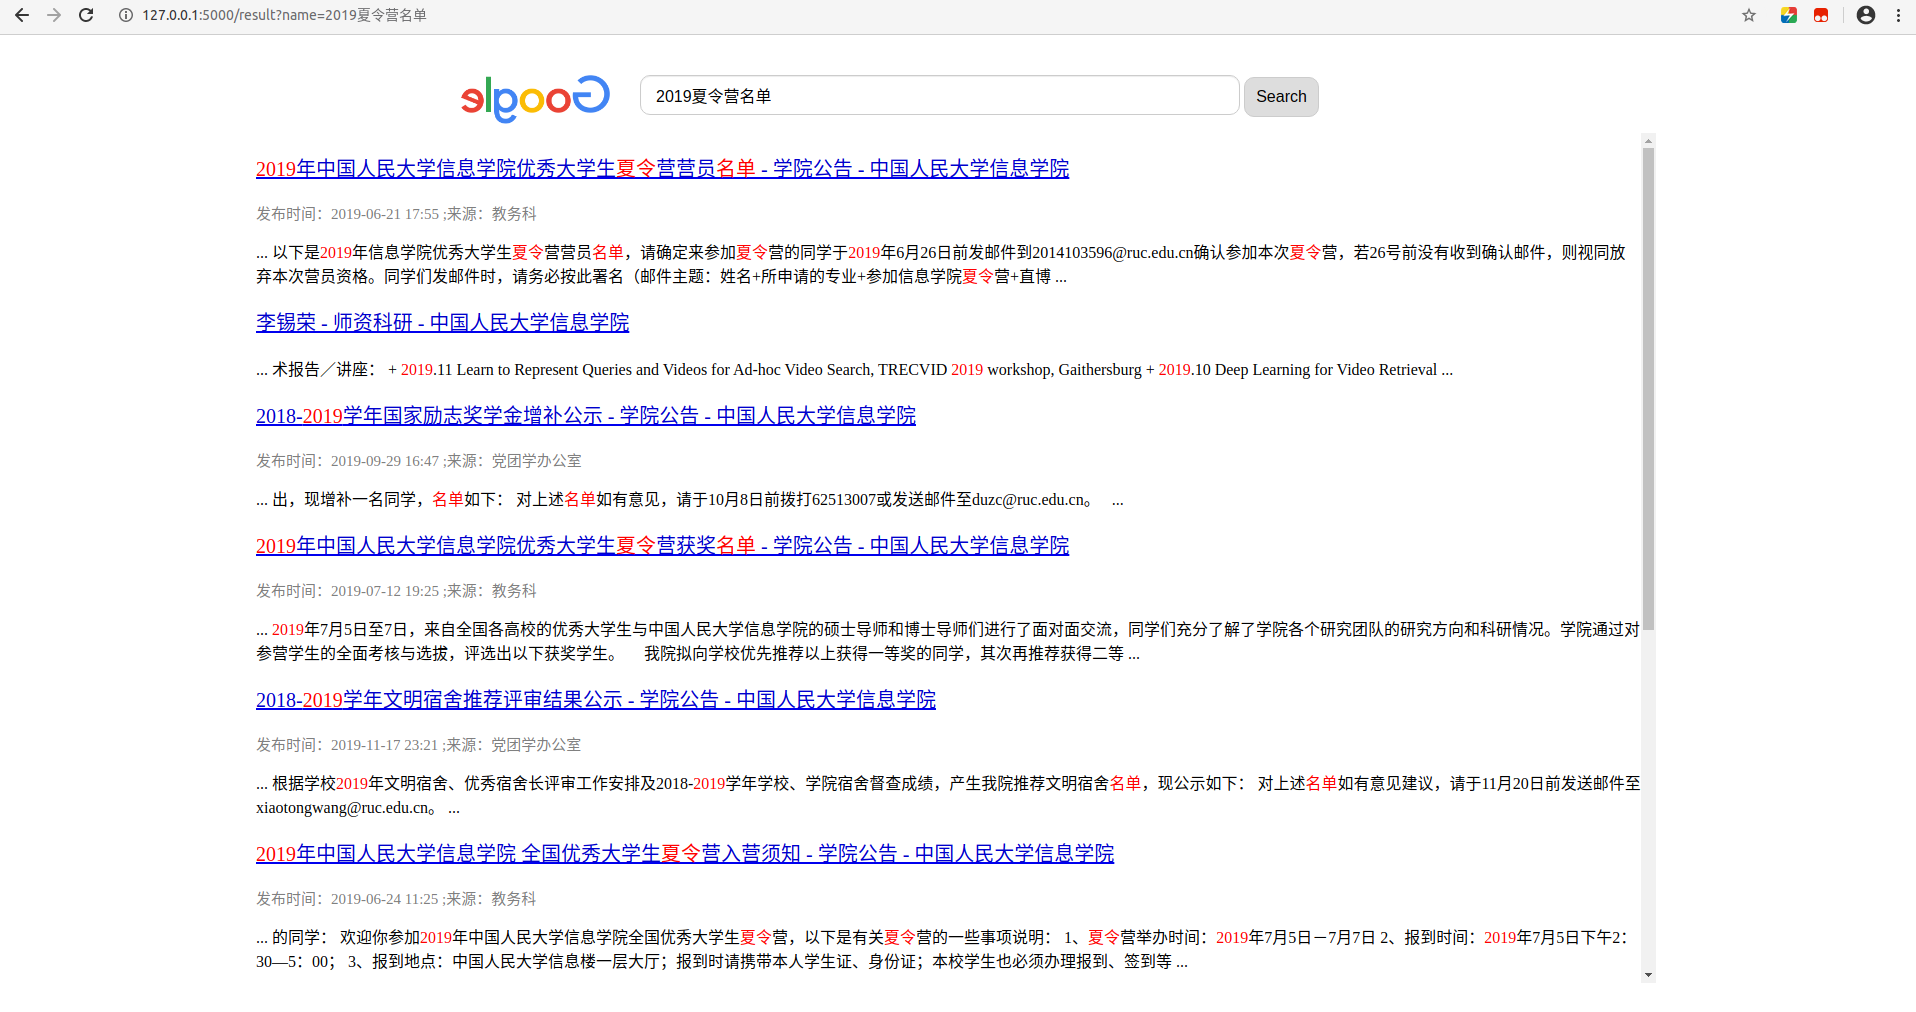
\includegraphics[width=1\textwidth, height=0.6\textheight]{example2.png}
	\end{center}
\end{frame}

\begin{frame}
\frametitle{Example-3}
\begin{center}
	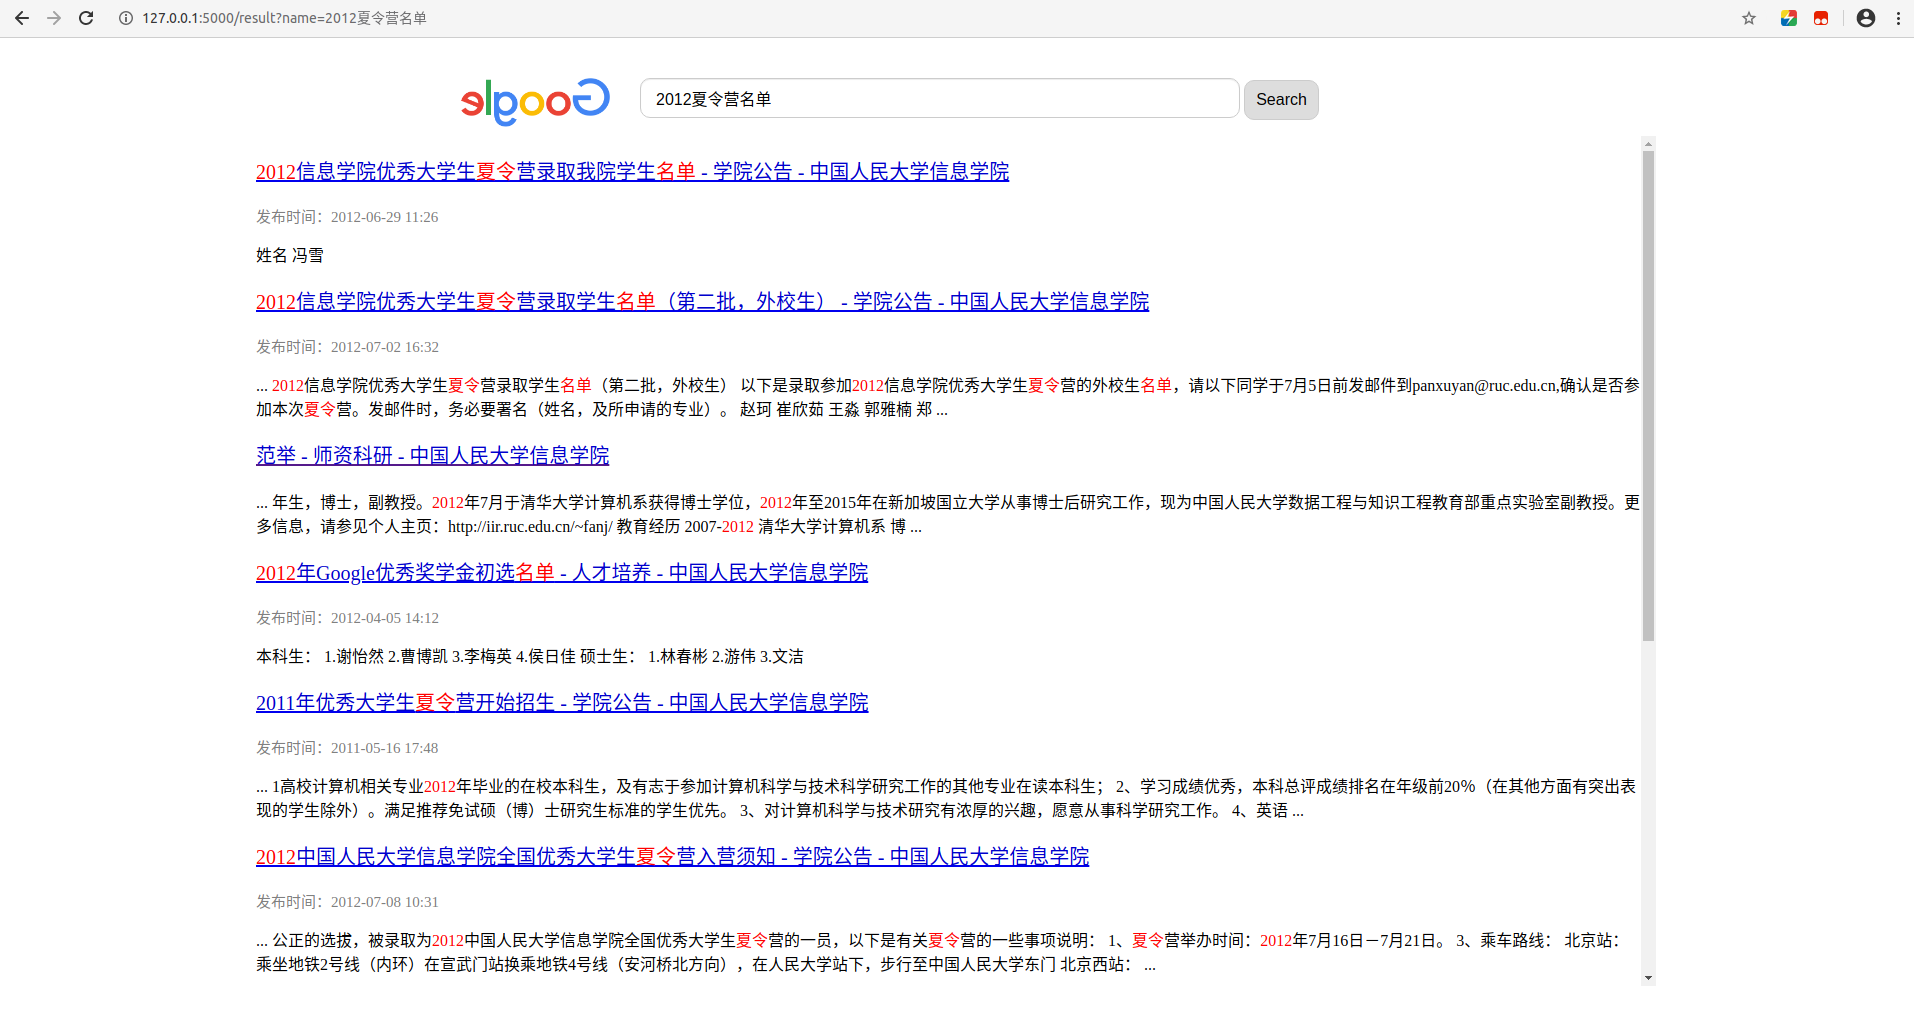
\includegraphics[width=1\textwidth, height=0.6\textheight]{example3.png}
\end{center}
\end{frame}

\begin{frame}
	\Large
	\centering
	Thank you for listening!
\end{frame}

\end{document}